\documentclass[a4paper, 11pt]{article}
\usepackage[english]{babel}
\usepackage[top=2cm,bottom=2cm,left=2cm,right=2cm]{geometry}
\usepackage[utf8]{inputenc}
\usepackage{import}
\usepackage{float}
\usepackage{subfigure}
% \usepackage{subfig}
\usepackage[pdftex]{graphicx}
% \usepackage{graphicx}
\usepackage{amssymb,amsmath,amsthm,amsfonts}
\usepackage{xspace}
\usepackage{tabularx}
\usepackage{indentfirst}
\usepackage{wrapfig,booktabs}
%\usepackage[small]{caption}
% \usepackage{subcaption}
\usepackage{eucal}
\usepackage{eso-pic}
\usepackage{hyperref}
\usepackage{url}
\usepackage{booktabs}
\usepackage{afterpage}
\usepackage{parskip}
\usepackage{listings}
\usepackage{fancyhdr}
\usepackage{textcomp}
\usepackage{cite}
\usepackage{multirow,multicol}
\usepackage{setspace}
\usepackage[version=4]{mhchem}
\usepackage{nicefrac}
\usepackage{siunitx}

\usepackage{caption}
\captionsetup{tableposition=top,font=small,width=0.8\textwidth}
%\usepackage[table]{xcolor}
\usepackage[arrowdel]{physics}
\usepackage{mathtools}
\usepackage{tablefootnote}
\usepackage{enumitem}

\setlist[description]{font={\scshape}} %style=unboxed,style=nextline
\usepackage{floatflt}
\usepackage{commath}
\usepackage{bm}
\usepackage{ifthen}
\usepackage{comment}
\usepackage[colorinlistoftodos,textsize=tiny]{todonotes}

\newcommand{\overbar}[1]{\mkern 1.5mu\overline{\mkern-1.5mu#1\mkern-1.5mu}\mkern 1.5mu}
\let\oldfrac\frac
\renewcommand{\frac}[3][d]{\ifthenelse{\equal{#1}{d}}{\oldfrac{#2}{#3}}{\nicefrac{#2}{#3}}}


\begin{document}

\title{Quantum Optics Lab report}
\author{Alessandro Lovo}

\maketitle

\begin{abstract}
  In this report, using the same experimental apparatus, three experiments regarding the quantum entanglement of photons will be performed: Entangled Quantum Key Distribution, Bell Inequality Violation and Quantum Tomography.
\end{abstract}


\section{Experimental apparatus}
  \begin{figure}[H]
    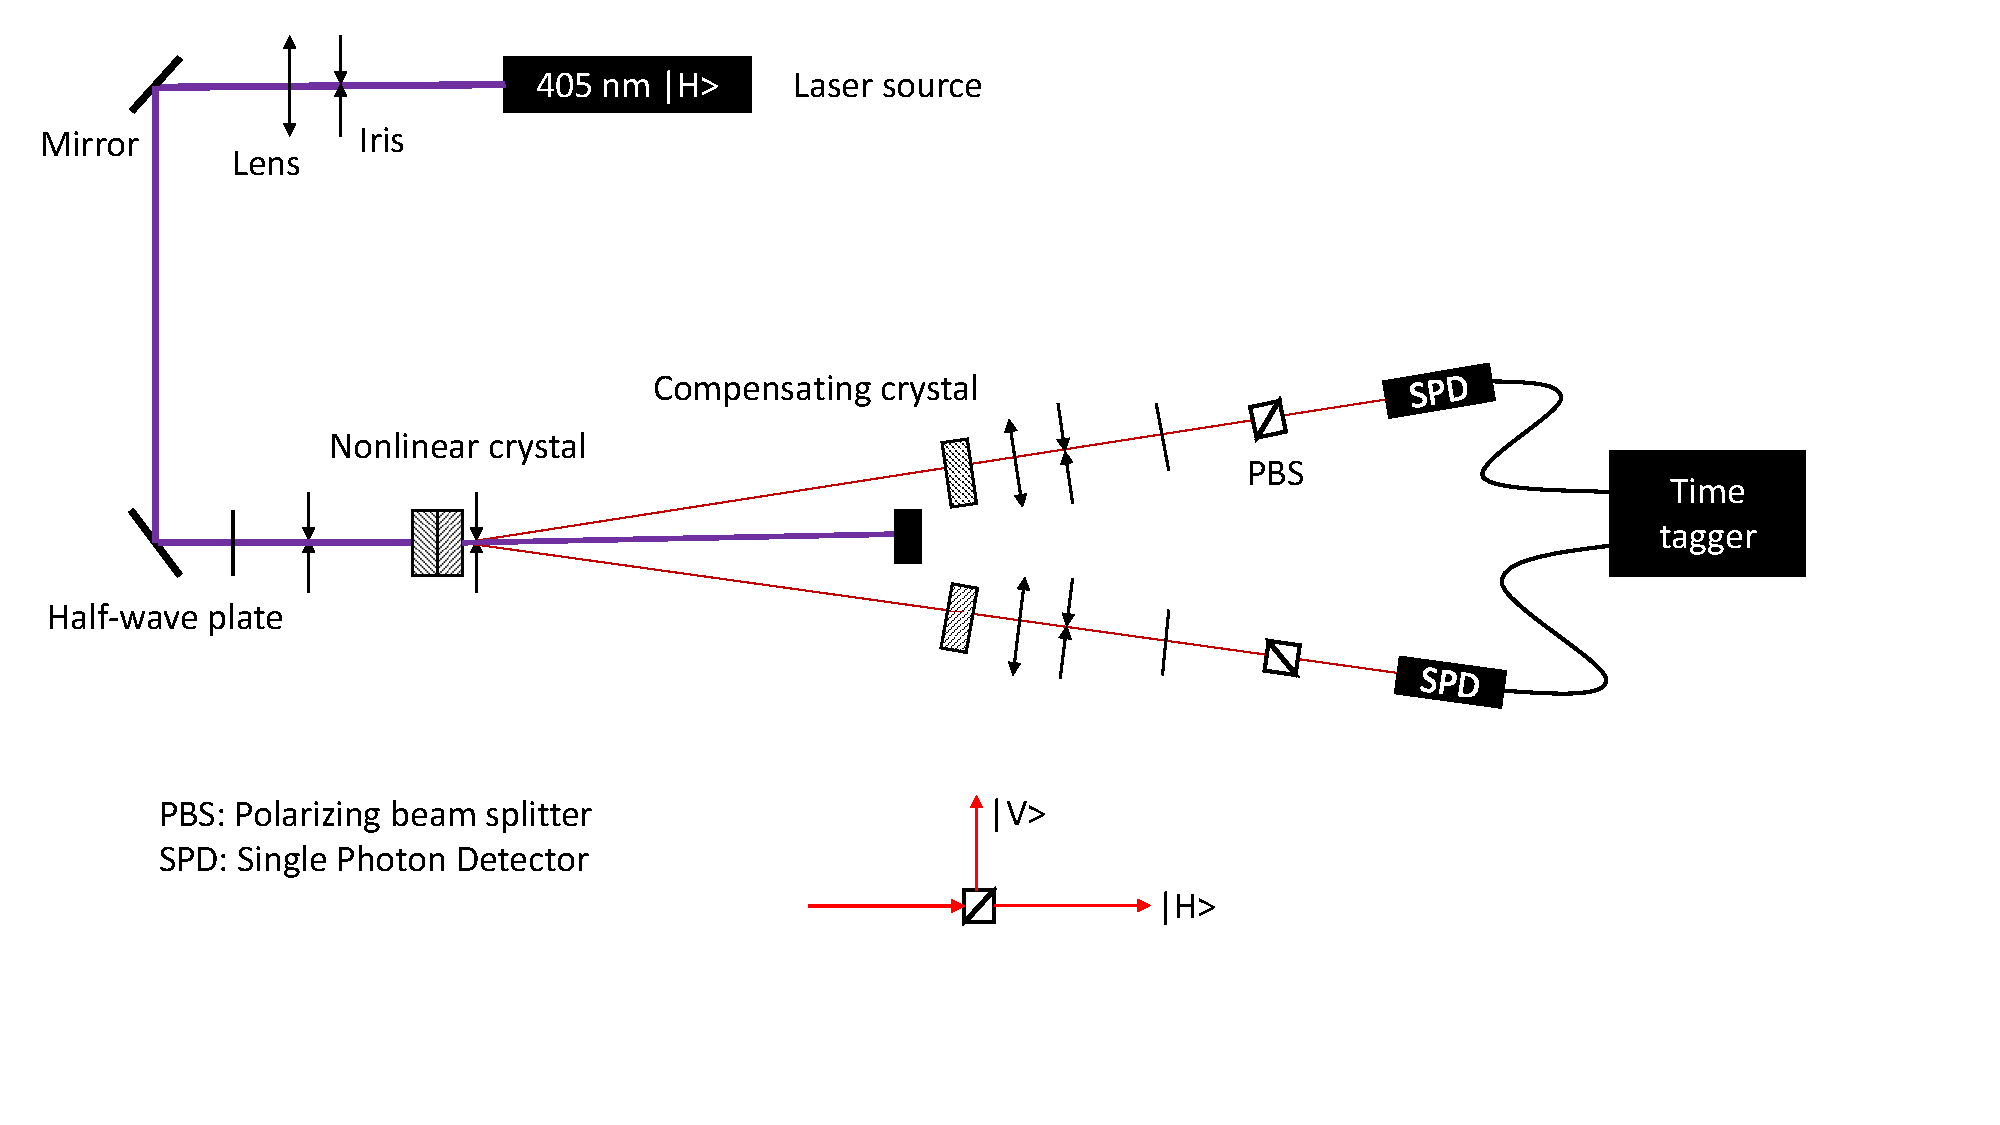
\includegraphics[width=1.0\textwidth]{img/apparatus.pdf}
    \caption{Schematics of the experimental apparatus.}
    \label{fig:apparatus}
  \end{figure}
  The schematics of the experimental apparatus are reported in fig \ref{fig:apparatus}: the source is a 405 \si{\nano\meter} laser whose beam is focused onto a nonlinear type II crystal obtained by sticking together two type I crystals with perpendicular optical axes. The laser emits light horizontally polarized ($\ket{H}$) and the two nonlinear crystals have a small chance ($\sim 10^{-7}$) of converting a photon into a pair of photons: if $\ket{V}$ is the vertical polarization, the conversion reads as:
  \begin{gather*}
    \ket{H} \xrightarrow[]{\text{crystal 1}} \ket{VV} \quad
    \ket{V} \xrightarrow[]{\text{crystal 2}} \ket{HH}
  \end{gather*}
  Using the first half-wave plate the polarization of the beam is rotated to the diagonal state $\ket{D} = \frac{\ket{H} + \ket{V}}{\sqrt{2}}$, so when it impinges on the two crystals the exiting pair is in the entangled state $\ket{\phi^+} = \frac{\ket{HH} + \ket{VV}}{\sqrt{2}}$. However since the conversion is due to two type I crystals in order to not be able to distinguish which one did the conversion, two compensating crystals are introduced on the optical path. After some focusing the two beams hit the measuring device: a half-wave plate, a polarizing beam splitter (PBS) and a single photon detector (SPD).
  By tuning the angle $\alpha$ of the half-wave plate it is possible to measure any linear polarization $\ket{\theta} = \cos{\theta}\ket{H} + \sin{\theta}\ket{V}$ with the simple relation $\theta = 2\alpha$.
  The signals of the SPDs are sent to a time tagger in order to be able to do an a-posteriori coincidence analysis.

  \par{Coincidence analysis}
  The raw data of an acquisition consist of a list of timetags corresponding to the clicks of each of the two detectors expressed in timesteps of the time tagger $\tau = 80.955\si{.\pico\second}$. To extract the coincidences from it, first a histogram of the time differences between the two detectors is plotted and fitted with a gaussian with centroid $\mu$ and dispersion $\sigma$ (fig \ref{fig:hist}). At this point one can set a threshold $thr_{c} = 2\sigma$ for accepting coincidences, namely the number of coincidences $N$ is simply the number of points in the histogram for which $|\frac[f]{\Delta t}{\tau} - \mu| < thr_{c}$. To this value can be then assosciated a poissonian error $\sigma(N) = \sqrt{N}$.

  \begin{figure}[H]
    \centering
    \resizebox{0.7\textwidth}{!}{\import{img/}{coinc_hist_AA.pgf}}
    \caption{Example of histogram of the time differences between the two detectors; here both photons are measured in the state $\ket{A} = \ket{\frac[f]{-\pi}{4}}$. The red lines are drawn at $thr_c$.}
    \label{fig:hist}
  \end{figure}


  \section{Entangled Quantum Key Distribution}
    Following the protocol BBM92 Alice and Bob share a source of entangled photons (in our experiment Alice and Bob can be considered as the two measuring devices measuring the photon pairs) and will end up with a random secret shared key. The protocol can be summarized as follows:
    \begin{enumerate}
      \item \emph{Quantum Communication} For each photon they receive, Alice and Bob randomly and independently choose in which base to measure the polarization:
      \begin{gather*}
        \mathcal{B}_1 = \left\{ \ket{H}, \ket{V} \right\}
        \quad \text{or} \quad
        \mathcal{B}_2 = \left\{ \ket{D} = \ket{\frac[f]{\pi}{4}}, \ket{A} = \ket{-\frac[f]{\pi}{4}} \right\}.
      \end{gather*}
      Since the state of the pair is $\ket{\phi^+} = \frac{\ket{HH} + \ket{VV}}{\sqrt{2}} = \frac{\ket{DD} + \ket{AA}}{\sqrt{2}}$ for each measurement they have a 50\% chance of obtaining either result: result that can be coded, for example, as 0 if it is first element of the base and 1 if it is the second.
      \item \emph{Sifting} After all the measurements they communicate via a classical channel the sequence of bases used for the measurement, restricting to the data in which they both measured in the same base. So on average the lenght of the key halves.
      \item \emph{Parameter Estimation} Alice and Bob communicate to each other the results of the measurements of a portion (for example $r_s = 10\%$) of the sifted key to estimate the Quantum Bit Error Rate (QBER), namely the percentage of measurements in which they obtained a different result. The Qber can then be used to quantify the information that an eventual Evesdroppper has on the key.
      \item \emph{Error Correction} Classical protocol at the end of which Alice and Bob have the same key, but the Evesdroppper has still information on it.
      \item \emph{Privacy Amplification} Other classical protocol that allows Alice and Bob to extract from their shared key a shorter one on which the Evesdroppper has no information at all. With this step the lenght of the key gets multiplied by the secret key rate
      \begin{equation*}
        r = 1 - h_2(QBER[\mathcal{B}_1]) - h_2(QBER[\mathcal{B}_2])
      \end{equation*}
      where
      \begin{equation*}
        h_2(x) = -x\log_2x - (1 - x)\log_2(1 - x)
      \end{equation*}
      is the Shannon entropy.
      Clearly as the QBER increases, $r$ decreases and when $r < 0$ it is impossible to extract a secure key. The relationship between $r$ and the QBER is plotted in fig \ref{fig:r_vs_qber}.
      If one considers also the losses in key lenght due to sifting and parameter estimation the ratio between number of bits in the final key and number of pair of photons measured is $\frac{1}{2} (1 - r_s) r$.
    \end{enumerate}

    \begin{figure}[H]
      \centering
      \resizebox{0.7\textwidth}{!}{\import{img/}{r_vs_qber.pgf}}
      \caption{Secret key rate as a function of the QBER in the tw bases. The red dot represents the experimental point found later.}
      \label{fig:r_vs_qber}
    \end{figure}

    \subsection{Experimental data}
      In the experiment we performed the focus is on the computation of the QBER and subsequently the estimation of the secret key rate. To do so we rotated the two half-wave plates in order to measure the pair of photons in the states reported in tab \ref{tab:QKD_coinc} acquiring for each configuration a dataset of around 15 s. In order to have a correct normalization, all datasets have been cropped in order to have the same temporal lenght of the shortest one: 14.016 s.

      \begin{table}[H]
        \centering
        \begin{tabular}{cccccccc}
          \toprule
          Configuration & Coincidences \\
          \midrule
          AA & $4440 \pm 70$ \\
          AD & $140 \pm 10$ \\
          DA & $120 \pm 10$ \\
          DD & $4270 \pm 70$ \\
          \midrule
          HH & $4390 \pm 70$ \\
          HV & $21 \pm 4$ \\
          VH & $64 \pm 8$ \\
          VV & $4410 \pm 70$ \\
          \bottomrule
        \end{tabular}
        \caption{Number of coincidences}
        \label{tab:QKD_coinc}
      \end{table}

      From these data it is then possible to compute the two QBERs and hence the secret key rate. If $N_{HH}$ is the number of coincidences measured in configuration HH one gets the following:

      \begin{gather*}
        QBER[\mathcal{B}_1] = \frac{N_{HV} + N_{VH}}{N_{HH} + N_{HV} + N_{VH} + N_{VV}} =  0.010 \pm 0.001 \\
        QBER[\mathcal{B}_2] = \frac{N_{DA} + N_{AD}}{N_{DD} + N_{DA} + N_{AD} + N_{AA}} = 0.029 \pm 0.002 \\
        r = 1 - h_2(QBER[\mathcal{B}_1]) - h_2(QBER[\mathcal{B}_2]) = 0.73 \pm 0.01
      \end{gather*}


  \section{Bell test}
    With the same apparatus it is possible to perform a violation of the Bell inequalities thus proving experimentally that a hidden variable theory does not describe the physical world. To do so let us consider the two SPDs as two observers who are able to measure their photon in two bases.
    For the first observer the base used is denoted with $x$ while the result of the measurement can be denoted with $a$ and assumes value 0 if the photon is projected onto the first element of the base and 1 otherwise. Analogously for the second observer the two variables are denoted with $y$ for the choice of the base and $b$ for the result of the measurement.

    \begin{gather*}
      \mathcal{B}_1(x) =
      \begin{cases}
        \left\{ \ket{H}, \ket{V} \right\} & x = 0 \\
        \left\{ \ket{D}, \ket{A} \right\} & x = 1
      \end{cases}
      \qquad
      \mathcal{B}_2(y) =
      \begin{cases}
        \left\{ \ket{\frac[f]{\pi}{8}}, \ket{\frac[f]{5\pi}{8}} \right\} & y = 0 \\
        \left\{ \ket{-\frac[f]{\pi}{8}}, \ket{\frac[f]{3\pi}{8}} \right\} & y = 1
      \end{cases}
    \end{gather*}

    Similarly to what has been done in the previous experiment, we took 16 different measurement of coincidences (one for each combination of $x,y,a,b$) and cropping all the 16 datasets to the lenght of the shortest ($7.84 \si{.\second}$) we obtained the results in tab \ref{tab:Bell_coinc} where the number of coincidences is denoted as $N_{ab|xy}$.

    \begin{table}[H]
      \centering
      \begin{tabular}{cccccccc}
        \toprule
        $x$ & $a$ & $y$ & $b$ & $N_{ab|xy}$ \\
        \midrule
        0 & 0 & 0 & 0 & $3460 \pm 60$ \\
        0 & 0 & 0 & 1 & $590 \pm 20$ \\
        0 & 1 & 0 & 0 & $710 \pm 30$ \\
        0 & 1 & 0 & 1 & $2850 \pm 50$ \\
        \midrule
        0 & 0 & 1 & 0 & $3300 \pm 60$ \\
        0 & 0 & 1 & 1 & $480 \pm 20$ \\
        0 & 1 & 1 & 0 & $380 \pm 20$ \\
        0 & 1 & 1 & 1 & $3360 \pm 60$ \\
        \midrule
        1 & 0 & 0 & 0 & $3290 \pm 60$ \\
        1 & 0 & 0 & 1 & $600 \pm 20$ \\
        1 & 1 & 0 & 0 & $760 \pm 30$ \\
        1 & 1 & 0 & 1 & $2960 \pm 50$ \\
        \midrule
        1 & 0 & 1 & 0 & $980 \pm 30$ \\
        1 & 0 & 1 & 1 & $2830 \pm 50$ \\
        1 & 1 & 1 & 0 & $3110 \pm 60$ \\
        1 & 1 & 1 & 1 & $730 \pm 30$ \\
        \bottomrule
      \end{tabular}
      \caption{Coincidences for the Bell test.}
      \label{tab:Bell_coinc}
    \end{table}

    From these coincidences one can define the probability of each combination $x,y,a,b$ as
    \begin{equation*}
      P(a,b|x,y) := \frac{N_{ab|xy}}{\sum_{a'b'}N_{a'b'|xy}}
    \end{equation*}
    and from those probabilities the quantities
    \begin{equation*}
      \langle E_{xy} \rangle := P(0,0|x,y) + P(1,1|x,y) - P(0,1|x,y) - P(1,0|x,y)
    \end{equation*}
    that result to be
    \begin{gather*}
      \langle E_{00} \rangle = 0.659 \pm 0.009 \qquad \langle E_{01} \rangle = 0.772 \pm 0.007 \\
      \langle E_{10} \rangle = 0.643 \pm 0.009 \qquad \langle E_{11} \rangle = -0.55 \pm 0.01
    \end{gather*}

    At this point one can define the quantity
    \begin{equation*}
      CHSH := \langle E_{00} \rangle + \langle E_{01} \rangle + \langle E_{10} \rangle - \langle E_{11} \rangle = 2.63 \pm 0.02
    \end{equation*}
    that in a model with hidden variables is limited by $CHSH < 2$, while for quantum mechanics the condition is relaxed to $CHSH < 2\sqrt{2} \approx 2.83$. The result we found is around $36\sigma$ beyond the hidden variable limit and well within the quantum one, thus proving that the hidden variable theory is incompatible with experimental results.













\end{document}
